\chapter{Background}

\section{Cloud computing}

Cloud computing is a model of providing computing resources as a service, which
is now very well established. At its core, it makes concentrated, shared compute
resources available on demand, via the network. These resources are owned and
controlled by a cloud service provider and made available remotely to users -
clients who thus achieve lower up front cost computing infrastructure,
flexibility, scalability, reduced deployment times and simplified infrastructure
administration \cite{wiki:cloud}.

We can distinguish three primary cloud service models, through which the
underlying resources are offered, as shown in fig. \ref{fig:cloud}
\cite{nist-cloud}:
\begin{description}
    \item[Infrastructure-as-a-Service (IaaS)] which provides compute, storage
          and networking resources, such as virtual machines, storage drives,
          virtual networks and load balancers. This model offers the lowest
          level of abstraction but the greatest flexibility to the users.
    \item[Platform-as-a-Service (PaaS)] where the users are able to develop
          their applications, assuming the ``environment'' in which those will
          be executed. Fundamentally, this model provides a higher level
          service, in the sense that they are not burdened with managing
          components such as the operating system or runtime system, allowing
          them to focus on the application instead.
    \item[Software-as-a-Service (SaaS)] presenting the highest level of
          abstraction from the infrastructure. According to this model, the
          users are granted access to applications which are fully managed by
          the provider, from the underlying infrastructure to the configuration
          of the application itself. Examples of this are email services,
          project management and office suite applications such as document and
            spreadsheet editors.
\end{description}

\begin{figure}
    \centering
    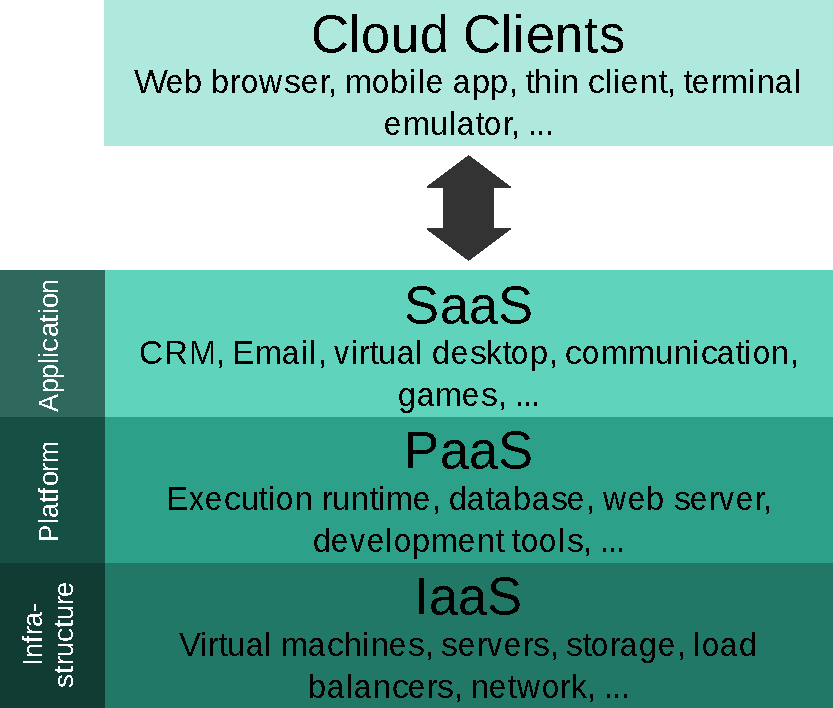
\includegraphics[scale=0.8]{cloud-layers}
    \caption[Cloud service models]{Cloud service models. Source
        \href{https://commons.wikimedia.org/wiki/File:Cloud_computing_layers.svg}{Wikimedia Commons}.}
    \label{fig:cloud}
\end{figure}

One model which emerged more recently, attracting a lot of user attention is
the so called serverless or Function-as-a-Service (FaaS). This resembles PaaS
(it could be considered part of it, or an evolved form), since as the name
suggests, it completely takes away the duty of server management from the users.
The emphasized technical aspects include automatic scalability from zero as well
as instant reaction to load fluctuations thanks to rapid startup and termination
of application instances \cite{cloudflare-serverless}. One of the drawbacks of
serverless is that only some applications fit this model, allowing them to
benefit from the above \cite{serverless, spec-serverless}.

\section{Virtualization}

The technology at the foundation of the cloud is that of virtualization. This
adds an abstraction layer over the physical compute infrastructure, enabling
the mapping of one (typically large) physical machine (host) to more, smaller
virtual machines (guests), created, modified, moved and deleted dynamically
through software \cite{wiki:hw-virtualization}.

Regarding the requirements for software running as guest, we discern two cases:
\begin{description}
    \item[Full virtualization] where the guest is not aware of running inside a
          virtual machine. This way, no changes are required for software
          written for physical machines to execute in virtual ones.
    \item[Paravirtualization] where the guest is modified specifically for
          execution in a virtual machine.
\end{description}
Virtualization has been around for decades prior to the advent of the cloud. One
decisive point for the realization of the latter was the addition of hardware
support for it in the x86 architecture, which led to its efficient use, without
high demands from software \cite{virtualization-x86}. Unto that point,
virtualization on this highly popular architecture relied upon
paravirtualization techniques.

The responsibility for accomplishing virtualization lies with the hypervisor or
virtual machine monitor (VMM). This is usually software running on the host,
with elevated privileges. Its tasks include starting the virtual machines and
emulating the operations not permitted to them, mainly interacting with the
system's devices. The latter is normally implemented through the ``trap and
emulate'' technique, where some instructions during the virtual machine's
execution cause CPU traps, transferring control to the hypervisor code. That
in turn checks and executes the guest's operation, eventually returning control
back where it had stopped. This mechanism grants the hypervisor full control
over the (virtual) device model of the virtual machine \cite{wiki:hypervisor}.

Hypervisors are classified in two primary categories (fig.
\ref{fig:hypervisors}) \cite{popek74}:
\begin{description}
    \item[Type 1] which execute directly on top of the physical machine,
          assuming complete control over it, in addition to managing the virtual
          machines. Usually these hypervisors depend on a special-purpose guest,
          running with elevated privileges, to manage the machine's devices,
          having the necessary drivers. The best known, free software such
          hypervisor is Xen \cite{xen}.
    \item[Type 2] which execute as part of a typical operating system, only in
          charge of starting and monitoring the virtual machines, while the host
          is managed by the operating system as usual. In this category it is
          customary for every guest to be a regular process from the host's
          perspective. The most popular free software representative of this
          category is \qemu{} \cite{qemu} (usually in combination with KVM
          \cite{kvm} to provide hardware acceleration).
\end{description}

\begin{figure}
    \centering
    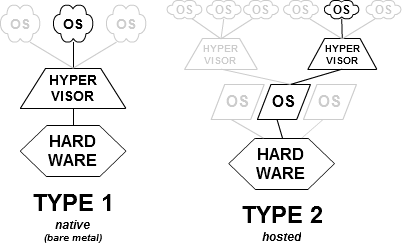
\includegraphics[scale=0.7]{hypervisors}
    \caption[Hypervisor types]{Hypervisor types. Source
        \href{https://commons.wikimedia.org/wiki/File:Hyperviseur.png}{Wikimedia Commons}.}
    \label{fig:hypervisors}
\end{figure}

\section{Unikernels}

In the common virtualization use case, the software supporting an application
can be viewed as (see fig. \ref{fig:components-vm}):
\begin{itemize}
    \item On the host (kernel space) runs a general-purpose operating system
          with direct access to the physical machine's resources and assuming
          responsibility over them.
    \item On the host (typically user space) also runs the hypervisor, assuming
          the duty of managing the virtual machines which correspond to the
          system.
    \item On the guest (kernel space) again runs an instance of a
          general-purpose operating system. This is responsible for the
          resources allocated to the virtual machine by the hypervisor.
    \item On the guest (user space) runs the application, frequently in
          conjunction with components like third-party libraries and runtime
          systems.
\end{itemize}
Ths software stack contains duplication and high complexity, two elements
commonly at fault for problems such as sub-optimal resource usage, reduced
performance due to overheads (e.g. mode switches) in the overall system
operation and security hazards due to the software's size, of which a good part
is unnecessary (e.g. guest drivers).
% TODO OPT: any citation?

\begin{figure}
    \centering
    \begin{subfigure}[b]{0.3\textwidth}
        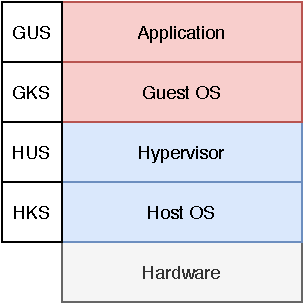
\includegraphics[width=\textwidth]{components-vm}
        \caption{Typical VM}
        \label{fig:components-vm}
    \end{subfigure}
    \begin{subfigure}[b]{0.3\textwidth}
        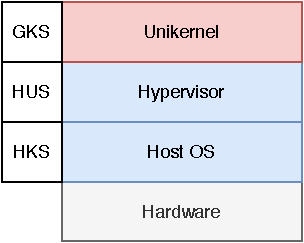
\includegraphics[width=\textwidth]{components-unikernel}
        \caption{Unikernel}
        \label{fig:components-unikernel}
    \end{subfigure}
    \begin{subfigure}[b]{0.3\textwidth}
        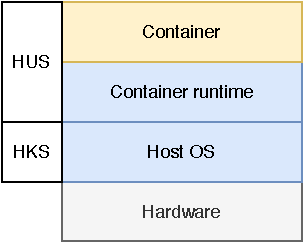
\includegraphics[width=\textwidth]{components-container}
        \caption{Container}
        \label{fig:components-container}
    \end{subfigure}
    \caption[Comparison between ``classic'' virtual machine arrangement,
        unikernel and container]{Comparison between ``classic'' virtual machine
        arrangement, unikernel and container, with a type 2 hypervisor. Where
        HKS=Host Kernel Space, HUS=Host User Space, GKS=Guest Kernel Space and
        GUS=Guest User Space.}
    \label{fig:vm-unikernel-container}
\end{figure}

A modern attempt at rectifying the above problem are unikernels \cite{mirageos}.
These are executable machine images comprising of an application bundled with
all necessary dependencies for its execution, from the likes of libraries and
runtime systems to network stacks and device drivers. All of these are situated
in a common, flat address space, as seen in fig. \ref{fig:components-unikernel}.
Unikernels are thus special-purpose kernels, built to run a single application
in a virtual machine, considering that virtual machines are regularly employed
to serve just a single application.

Unikernels are established on the older idea of library operating systems, which
were introduced with the innovative at the time and very relevant today
exokernels \cite{exokernel}. In a library operating system the majority of the
functionalities traditionally offered as part of a monolithic kernel (e.g. file
systems and networking) are extracted from it, becoming independent elements in
the form of libraries which accompany an application. This rearrangement grants
the application the liberty of choosing which of these elements in requires, as
well as which implementation of each it prefers. Therefore, the application
can optimize its operation through said choices, but at the same time is
burdened with this extra duty.

A big hurdle in implementing unikernels is the diversity of devices and
consequently drivers necessary to operate them. This is overcome thanks to the
hypervisors' device model, encompassing few, common and well documented devices.
Another obstacle is the complexity associated with matching the various
components together to create the final executable image. There are numerous
solutions proposed to this, each forming a ``unikernel framework''. Virtually
all of those are free software projects, each providing a set of libraries for
inclusion by the user applications, as well as the tools necessary for building
the images. Each of these frameworks typically takes one of two principal
approaches:
\begin{itemize}
    \item Clean-slate, providing custom APIs. In this case, both library and
          application code is written in the same programming language. A major
          downside to this approach is that the applications need to be written
          from scratch in the language and using the API of the respective
          framework.
    \item Compatible, providing standard interfaces (e.g. POSIX), which allows
          running existing applications with minimum to no modifications,
          independently of any programming language (binary compatibility). In
          this case, the biggest tradeoff is the commitment to legacy
          interfaces, often hindering taking full advantage of the unikernel
          potential.
\end{itemize}
For example, in the first category one finds MirageOS \cite{mirageos} and
IncludeOS \cite{includeos}, whereas in the second we note RumpRun
\cite{rumprun}, \osv{} \cite{osv} and HermiTux \cite{hermitux}. Overall, there
are several unikernel frameworks, varying in popularity (with none prevailing),
maintenance status (from active to practically abandoned) and origins (academic,
corporate-backed or personal projects).

% TODO OPT: Mention edge use case for unikernels? (not here necessarily)

\subsection{\osv{}}

\osv{} is a unikernel framework supporting applications written for linux,
while offering its own API which new applications can opt to use \cite{osv}.
It has been designed with the cloud in mind, in order to accommodate modern
applications most often encountered there. The project was started by Cloudius
Systems (later ScyllaDB) but lately it has been maintained and enhanced by a
small team of volunteers. It is made available under the terms of the BSD
software license. Its community makes use of a mailing list%
\footnote{\url{https://groups.google.com/forum/\#!forum/osv-dev}} for its
development: submitting patches, code reviews and general discussion.

Although it is mostly written in C++, also incorporating C code from other
projects, this imposes no restriction on the applications it supports, as long
as those don't make use of operations that by nature are not applicable in
unikernels: system calls in the family of \texttt{fork()} and \texttt{exec()}.
Moreover, it is supported on several hypervisors, including \qemu{}/KVM,
Xen and firecracker \cite{firecracker}. As a general note, it is one of the most
advanced unikernels in terms of features, and more heavy-weight as a result of
that.

Regarding file systems, \osv{} offers many choices. First of all, it boasts
a complete virtual file system (VFS), based on that of Prex \cite{prex}. Beneath
that are implementations of various file systems, which can be grouped in
two categories:
\begin{itemize}
    \item Pseudo-file systems, corresponding to those of linux: devfs, procfs,
          sysfs and ramfs.
    \item Conventional file systems: ZFS (based on FreeBSD's implementation),
          rofs (custom, read-only file system with simple caching functionality)
          and NFS (powered by libnfs \cite{libnfs}).
\end{itemize}

% TODO OPT: More technical: virtual memory, virtual file system, network stack,
% aarch64, musl.

\subsection{Alternatives}

As expected, there have been alternative approaches to the problem of bloat in
the virtualized software stack. By far the most popular at this point is that of
containers. These belong to the broad class of OS-level virtualization
\cite{wiki:os-level-virtualization} (see fig. \ref{fig:components-container}).

There exist multiple techniques for implementing containers, most of which rely
on linux kernel mechanisms, like cgroups and namespaces, to achieve isolation
between separate containers. What's common among all container technologies is
that applications running in all containers on the same host share the same
kernel instance. One could say that in this case there is a single kernel but
many user spaces.

Probably the chief advantage of containers is that they are a lot ``lighter''
than virtual machines: much lower startup times (compared to a VM with a
general-purpose guest), greater flexibility and lower resource usage, resulting
in higher density (instances running concurrently on the same physical machine).
Their weakest point is that they offer much weaker isolation than virtual
machines, due to the common kernel serving them \cite{lightvm}.

% TODO OPT: Αll other approaches (lw virt, user-space kernels).

% TODO OPT: Compare native, legacy virtual, unikernel and container execution in
% terms of flexibility, security (separation) and efficiency / scalability.

\section{Shared file systems}

``Classic'' file systems are implemented over block devices (``disks'')
connected via a local system bus. The software comprising them is usually part
of an operating system kernel which assumes it is the exclusive user of the file
system for as long as that is mounted. This more often than not constitutes a
restriction with attempts to lift it since the advent of computer networking,
in order to allow concurrent use of a file system by more computers, rendering
it shared. The most prevalent and among the oldest representatives of shared
file systems is NFS (Network File System) \cite{nfs}, with this class of file
systems gaining many new members with the proliferation of distributed systems
in recent years.

Virtualization can be viewed as a special case of multiple, interconnected
machines: the host and the virtual machines running on it. The demand for a
file system shared between them is thus present and in fact very common due to
their coexistence on the same physical machine. After all, the host's file
system is yet another one of its resources, so it is expected for it to be
accessible by the guests.

Most solutions for host-guest shared file systems rely on the existing,
network file systems, not differentiating between this case and that of separate
hosts. This approach builds of course on the network connection between the
parts, fully reusing preexisting solutions. A popular example of shared file
system in the context of virtualization is VirtFS \cite{virtfs} which depends on
the 9P protocol \cite{9p}. Although the latter is a network protocol, VirtFS
does not use the network as its transport layer, granting it improved
performance.

It is worth mentioning that in the case of containers access to a file system
shared with the host is also in high demand. One way this is accomplished in
Docker \cite{docker} (by far the most prevalent container runtime) is through
bind mounts \cite{docker:bind-mounts}, taking advantage of the common kernel to
mount a host directory in the container's file system.

\section{\viofs{}}

The shared memory underlying both host and guests is an element not fully taken
advantage of by current shared file systems. Virtio-fs \cite{virtiofs-website}
sets out with the goal of changing that. Its differentiating factor is that it
is not dependent on the network at the transport layer (using virtio instead),
neither at the protocol layer (where it opts for FUSE). These two choices allow
for better performance as well as local file system semantics, which manifests
e.g. in coherence issues.

The existing \viofs{} implementation in \qemu{} is distinctive in its
architecture. Whereas device implementation is usually fully contained inside
\qemu{}, here a significant part is split in the so-called virtiofsd (\viofs{}
daemon), a separate process handling all file system operations on the host,
while \qemu{} is left with the task of implementing the virtual device. On one
hand, has the merit of higher security, since virtiofsd can be sandboxed with
the host's mechanisms (namespaces, seccomp). On the other hand, it is modular,
facilitating easy switching between different virtiofsd implementations (e.g.
with one backed by a distributed file system instead of the host's local file
system). Splitting the implementation in separate processes is made possible by
the host-user protocol \cite{vhost-user}, which evolves the idea of vhost in
\qemu{} \cite{stefanha:vhost}. Pushing devices out of the VMM has many
advantages and is expected to be favored in the future
\cite{stefanha:out-of-process-dev}.

\subsection{Virtio}

Virtio is a standard specifying devices exclusively for virtualized environments
\cite{virtio}. It enjoys wide support and is considered the de facto solution
to the problem of fragmentation in virtual device models. Offering an efficient
and extendable mechanism, it builds on physical device terminology and
mechanisms, thus assisting in new support for it and enabling reuse of existing
driver code in guests.

The standard consists mainly of two notions:
\begin{description}
    \item[The transport layer] which defines a generic way for device discovery,
          configuration and normal operation (bidirectional data transfer). The
          latter is achieved via so-called ``virtqueues'', relying on the shared
          memory between guest and hypervisor. The transport layer, initially
          given an abstract specification, is specialized by three
          implementations: PCI bus, memory-mapped I/O (MMIO) and channel I/O
          (used in cases of the IBM S/390 architecture).
    \item[The set of devices] which builds on the transport layer to specify
          for each device the available configuration fields, the number of
          virtqueues and the messages exchanged over those for its operation.
\end{description}

\subsection{FUSE}

FUSE (Filesystem in Userspace) is a protocol introduced in linux to enable
file system implementations in user space instead of inside the kernel
\cite{fuse}. As made clear in fig. \ref{fig:fuse}, the file system operations
are carried out by a user space daemon communicating with the kernel according
to the protocol via a special character device (\texttt{/dev/fuse}). When the
kernel receives VFS requests corresponding to a FUSE file system, it forwards
them to the appropriate daemon which acts as a backend.

\begin{figure}
    \centering
    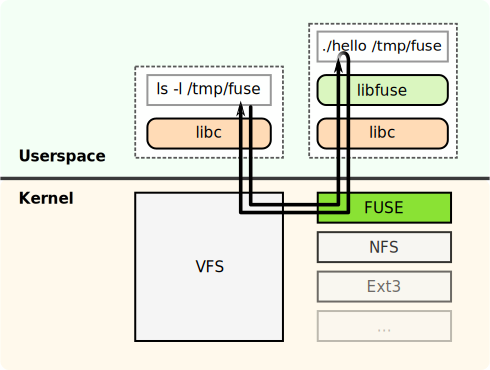
\includegraphics[width=\textwidth]{fuse}
    \caption[FUSE architecture in linux]{FUSE architecture in linux. By
        Sven (\url{https://commons.wikimedia.org/wiki/User:Sven}) licensed under
        CC-BY-SA 3.0
        (\url{https://creativecommons.org/licenses/by-sa/3.0/legalcode}).
        Source
        \url{https://commons.wikimedia.org/wiki/File:FUSE_structure.svg}.}
    \label{fig:fuse}
\end{figure}

In the context of \viofs{}, FUSE is utilized for communicating the file system
requests to the device. Hence its architecture resembles the classic FUSE
architecture, with the difference that the client is the guest instead of the
kernel, while communication is performed through virtio rather than the FUSE
character device. In practice though, \viofs{} and regular FUSE are incompatible
because \viofs{} incorporates modifications and extensions to the FUSE protocol.
Moreover, the security model differs (it is essentially inverted), with the
client (the guest) being untrusted in \viofs{}, whereas in FUSE it is the other
way round (by default there is trust in the kernel the daemon is running on).
The latter translates in safer request handling in a \viofs{} device backend
than in a FUSE backend.

% TODO OPT: Protocol description

\subsection{DAX window}

For the file read and write operations, FUSE utilizes the FUSE\_READ and
FUSE\_WRITE requests respectively. These involve copying the data and in the
case of \viofs{} ensue VM exits. Since these are operations at the core of the
data path, it is crucial for them to be optimized. To that end, \viofs{}
introduces the DAX window: a ``window'' of memory shared between the host and
the guest where file contents are mapped, providing the guest with direct access
on them. This results in skipping the copying (and bypassing the guest page
cache in the case of linux guests), while not every read or write operation
implies suspending the virtual machine's execution.

\begin{figure}
    \centering
    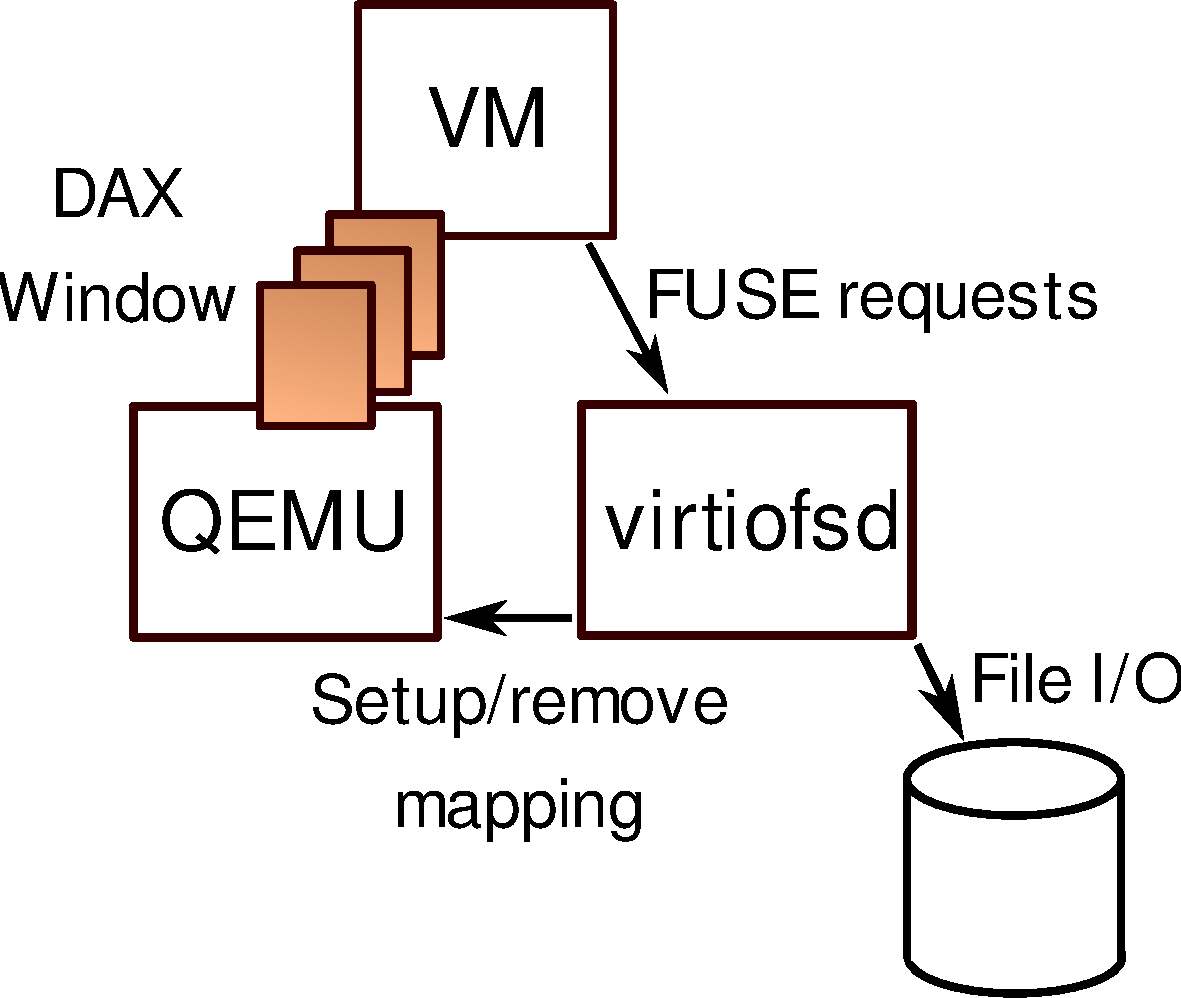
\includegraphics[scale=0.5]{dax-architecture}
    \caption[DAX window architecture in \viofs{}]{DAX window architecture in
        \viofs{}. By Stefan Hajnoczi (\url{https://vmsplice.net/}) licensed
        under CC-BY-SA 4.0
        (\url{https://creativecommons.org/licenses/by-sa/4.0/legalcode}).
        Source
        \url{https://gitlab.com/virtio-fs/virtio-fs.gitlab.io/-/blob/master/architecture.svg}.}
    \label{fig:dax-architecture}
\end{figure}

% TODO OPT: DAX subsystem in Linux, pmem

For realizing the DAX window functionality, initially the FUSE protocol is
extended with messages for establishing and removing mappings. The guest
dispatches these messages to virtiofsd, which carries out all necessary checks
and instructs \qemu{} to eventually perform the actual operation (establishing
or removing a mapping). See also fig. \ref{fig:dax-architecture}.
